% Options for packages loaded elsewhere
\PassOptionsToPackage{unicode}{hyperref}
\PassOptionsToPackage{hyphens}{url}
\PassOptionsToPackage{dvipsnames,svgnames,x11names}{xcolor}
%
\documentclass[
  letterpaper,
  DIV=11,
  numbers=noendperiod]{scrartcl}

\usepackage{amsmath,amssymb}
\usepackage{iftex}
\ifPDFTeX
  \usepackage[T1]{fontenc}
  \usepackage[utf8]{inputenc}
  \usepackage{textcomp} % provide euro and other symbols
\else % if luatex or xetex
  \usepackage{unicode-math}
  \defaultfontfeatures{Scale=MatchLowercase}
  \defaultfontfeatures[\rmfamily]{Ligatures=TeX,Scale=1}
\fi
\usepackage{lmodern}
\ifPDFTeX\else  
    % xetex/luatex font selection
\fi
% Use upquote if available, for straight quotes in verbatim environments
\IfFileExists{upquote.sty}{\usepackage{upquote}}{}
\IfFileExists{microtype.sty}{% use microtype if available
  \usepackage[]{microtype}
  \UseMicrotypeSet[protrusion]{basicmath} % disable protrusion for tt fonts
}{}
\makeatletter
\@ifundefined{KOMAClassName}{% if non-KOMA class
  \IfFileExists{parskip.sty}{%
    \usepackage{parskip}
  }{% else
    \setlength{\parindent}{0pt}
    \setlength{\parskip}{6pt plus 2pt minus 1pt}}
}{% if KOMA class
  \KOMAoptions{parskip=half}}
\makeatother
\usepackage{xcolor}
\setlength{\emergencystretch}{3em} % prevent overfull lines
\setcounter{secnumdepth}{-\maxdimen} % remove section numbering
% Make \paragraph and \subparagraph free-standing
\makeatletter
\ifx\paragraph\undefined\else
  \let\oldparagraph\paragraph
  \renewcommand{\paragraph}{
    \@ifstar
      \xxxParagraphStar
      \xxxParagraphNoStar
  }
  \newcommand{\xxxParagraphStar}[1]{\oldparagraph*{#1}\mbox{}}
  \newcommand{\xxxParagraphNoStar}[1]{\oldparagraph{#1}\mbox{}}
\fi
\ifx\subparagraph\undefined\else
  \let\oldsubparagraph\subparagraph
  \renewcommand{\subparagraph}{
    \@ifstar
      \xxxSubParagraphStar
      \xxxSubParagraphNoStar
  }
  \newcommand{\xxxSubParagraphStar}[1]{\oldsubparagraph*{#1}\mbox{}}
  \newcommand{\xxxSubParagraphNoStar}[1]{\oldsubparagraph{#1}\mbox{}}
\fi
\makeatother

\usepackage{color}
\usepackage{fancyvrb}
\newcommand{\VerbBar}{|}
\newcommand{\VERB}{\Verb[commandchars=\\\{\}]}
\DefineVerbatimEnvironment{Highlighting}{Verbatim}{commandchars=\\\{\}}
% Add ',fontsize=\small' for more characters per line
\usepackage{framed}
\definecolor{shadecolor}{RGB}{241,243,245}
\newenvironment{Shaded}{\begin{snugshade}}{\end{snugshade}}
\newcommand{\AlertTok}[1]{\textcolor[rgb]{0.68,0.00,0.00}{#1}}
\newcommand{\AnnotationTok}[1]{\textcolor[rgb]{0.37,0.37,0.37}{#1}}
\newcommand{\AttributeTok}[1]{\textcolor[rgb]{0.40,0.45,0.13}{#1}}
\newcommand{\BaseNTok}[1]{\textcolor[rgb]{0.68,0.00,0.00}{#1}}
\newcommand{\BuiltInTok}[1]{\textcolor[rgb]{0.00,0.23,0.31}{#1}}
\newcommand{\CharTok}[1]{\textcolor[rgb]{0.13,0.47,0.30}{#1}}
\newcommand{\CommentTok}[1]{\textcolor[rgb]{0.37,0.37,0.37}{#1}}
\newcommand{\CommentVarTok}[1]{\textcolor[rgb]{0.37,0.37,0.37}{\textit{#1}}}
\newcommand{\ConstantTok}[1]{\textcolor[rgb]{0.56,0.35,0.01}{#1}}
\newcommand{\ControlFlowTok}[1]{\textcolor[rgb]{0.00,0.23,0.31}{\textbf{#1}}}
\newcommand{\DataTypeTok}[1]{\textcolor[rgb]{0.68,0.00,0.00}{#1}}
\newcommand{\DecValTok}[1]{\textcolor[rgb]{0.68,0.00,0.00}{#1}}
\newcommand{\DocumentationTok}[1]{\textcolor[rgb]{0.37,0.37,0.37}{\textit{#1}}}
\newcommand{\ErrorTok}[1]{\textcolor[rgb]{0.68,0.00,0.00}{#1}}
\newcommand{\ExtensionTok}[1]{\textcolor[rgb]{0.00,0.23,0.31}{#1}}
\newcommand{\FloatTok}[1]{\textcolor[rgb]{0.68,0.00,0.00}{#1}}
\newcommand{\FunctionTok}[1]{\textcolor[rgb]{0.28,0.35,0.67}{#1}}
\newcommand{\ImportTok}[1]{\textcolor[rgb]{0.00,0.46,0.62}{#1}}
\newcommand{\InformationTok}[1]{\textcolor[rgb]{0.37,0.37,0.37}{#1}}
\newcommand{\KeywordTok}[1]{\textcolor[rgb]{0.00,0.23,0.31}{\textbf{#1}}}
\newcommand{\NormalTok}[1]{\textcolor[rgb]{0.00,0.23,0.31}{#1}}
\newcommand{\OperatorTok}[1]{\textcolor[rgb]{0.37,0.37,0.37}{#1}}
\newcommand{\OtherTok}[1]{\textcolor[rgb]{0.00,0.23,0.31}{#1}}
\newcommand{\PreprocessorTok}[1]{\textcolor[rgb]{0.68,0.00,0.00}{#1}}
\newcommand{\RegionMarkerTok}[1]{\textcolor[rgb]{0.00,0.23,0.31}{#1}}
\newcommand{\SpecialCharTok}[1]{\textcolor[rgb]{0.37,0.37,0.37}{#1}}
\newcommand{\SpecialStringTok}[1]{\textcolor[rgb]{0.13,0.47,0.30}{#1}}
\newcommand{\StringTok}[1]{\textcolor[rgb]{0.13,0.47,0.30}{#1}}
\newcommand{\VariableTok}[1]{\textcolor[rgb]{0.07,0.07,0.07}{#1}}
\newcommand{\VerbatimStringTok}[1]{\textcolor[rgb]{0.13,0.47,0.30}{#1}}
\newcommand{\WarningTok}[1]{\textcolor[rgb]{0.37,0.37,0.37}{\textit{#1}}}

\providecommand{\tightlist}{%
  \setlength{\itemsep}{0pt}\setlength{\parskip}{0pt}}\usepackage{longtable,booktabs,array}
\usepackage{calc} % for calculating minipage widths
% Correct order of tables after \paragraph or \subparagraph
\usepackage{etoolbox}
\makeatletter
\patchcmd\longtable{\par}{\if@noskipsec\mbox{}\fi\par}{}{}
\makeatother
% Allow footnotes in longtable head/foot
\IfFileExists{footnotehyper.sty}{\usepackage{footnotehyper}}{\usepackage{footnote}}
\makesavenoteenv{longtable}
\usepackage{graphicx}
\makeatletter
\def\maxwidth{\ifdim\Gin@nat@width>\linewidth\linewidth\else\Gin@nat@width\fi}
\def\maxheight{\ifdim\Gin@nat@height>\textheight\textheight\else\Gin@nat@height\fi}
\makeatother
% Scale images if necessary, so that they will not overflow the page
% margins by default, and it is still possible to overwrite the defaults
% using explicit options in \includegraphics[width, height, ...]{}
\setkeys{Gin}{width=\maxwidth,height=\maxheight,keepaspectratio}
% Set default figure placement to htbp
\makeatletter
\def\fps@figure{htbp}
\makeatother

\KOMAoption{captions}{tableheading}
\makeatletter
\@ifpackageloaded{caption}{}{\usepackage{caption}}
\AtBeginDocument{%
\ifdefined\contentsname
  \renewcommand*\contentsname{Table of contents}
\else
  \newcommand\contentsname{Table of contents}
\fi
\ifdefined\listfigurename
  \renewcommand*\listfigurename{List of Figures}
\else
  \newcommand\listfigurename{List of Figures}
\fi
\ifdefined\listtablename
  \renewcommand*\listtablename{List of Tables}
\else
  \newcommand\listtablename{List of Tables}
\fi
\ifdefined\figurename
  \renewcommand*\figurename{Figure}
\else
  \newcommand\figurename{Figure}
\fi
\ifdefined\tablename
  \renewcommand*\tablename{Table}
\else
  \newcommand\tablename{Table}
\fi
}
\@ifpackageloaded{float}{}{\usepackage{float}}
\floatstyle{ruled}
\@ifundefined{c@chapter}{\newfloat{codelisting}{h}{lop}}{\newfloat{codelisting}{h}{lop}[chapter]}
\floatname{codelisting}{Listing}
\newcommand*\listoflistings{\listof{codelisting}{List of Listings}}
\makeatother
\makeatletter
\makeatother
\makeatletter
\@ifpackageloaded{caption}{}{\usepackage{caption}}
\@ifpackageloaded{subcaption}{}{\usepackage{subcaption}}
\makeatother

\ifLuaTeX
  \usepackage{selnolig}  % disable illegal ligatures
\fi
\usepackage{bookmark}

\IfFileExists{xurl.sty}{\usepackage{xurl}}{} % add URL line breaks if available
\urlstyle{same} % disable monospaced font for URLs
\hypersetup{
  pdftitle={Conjunto de Ejercicios},
  colorlinks=true,
  linkcolor={blue},
  filecolor={Maroon},
  citecolor={Blue},
  urlcolor={Blue},
  pdfcreator={LaTeX via pandoc}}


\title{Conjunto de Ejercicios}
\author{}
\date{}

\begin{document}
\maketitle


Recuerde que debe iniciar y terminar cada ejercicio escribiendo la
descripción del problema, y enfatizando la respuesta.

\subsection{Ejercicio 1}\label{ejercicio-1}

Use el método de bisección para encontrar soluciones precisas dentro de
(10\^{}\{-6\}) para \(x^3 - 7x^2 + 14x - 6 = 0\) en cada intervalo:\\
- a. ({[}0, 1{]})

\begin{Shaded}
\begin{Highlighting}[]
\KeywordTok{def}\NormalTok{ f(x):}
    \ControlFlowTok{return}\NormalTok{ x}\OperatorTok{**}\DecValTok{3} \OperatorTok{{-}} \DecValTok{7}\OperatorTok{*}\NormalTok{x}\OperatorTok{**}\DecValTok{2} \OperatorTok{+} \DecValTok{14}\OperatorTok{*}\NormalTok{x }\OperatorTok{{-}} \DecValTok{6}

\KeywordTok{def}\NormalTok{ bisection\_method(a, b, tol}\OperatorTok{=}\FloatTok{1e{-}6}\NormalTok{):}
    \ControlFlowTok{if}\NormalTok{ f(a) }\OperatorTok{*}\NormalTok{ f(b) }\OperatorTok{\textgreater{}=} \DecValTok{0}\NormalTok{:}
        \BuiltInTok{print}\NormalTok{(}\StringTok{"El teorema de valor intermedio no se cumple."}\NormalTok{)}
        \ControlFlowTok{return} \VariableTok{None}
    
    \ControlFlowTok{while}\NormalTok{ (b }\OperatorTok{{-}}\NormalTok{ a) }\OperatorTok{/} \DecValTok{2} \OperatorTok{\textgreater{}}\NormalTok{ tol:}
\NormalTok{        m }\OperatorTok{=}\NormalTok{ (a }\OperatorTok{+}\NormalTok{ b) }\OperatorTok{/} \DecValTok{2}
        \ControlFlowTok{if}\NormalTok{ f(m) }\OperatorTok{==} \DecValTok{0}\NormalTok{:}
            \ControlFlowTok{return}\NormalTok{ m}
        \ControlFlowTok{elif}\NormalTok{ f(a) }\OperatorTok{*}\NormalTok{ f(m) }\OperatorTok{\textless{}} \DecValTok{0}\NormalTok{:}
\NormalTok{            b }\OperatorTok{=}\NormalTok{ m}
        \ControlFlowTok{else}\NormalTok{:}
\NormalTok{            a }\OperatorTok{=}\NormalTok{ m}

    \ControlFlowTok{return}\NormalTok{ (a }\OperatorTok{+}\NormalTok{ b) }\OperatorTok{/} \DecValTok{2}

\CommentTok{\# Ejercicio 1.a: Intervalo [0, 1]}
\NormalTok{raiz1 }\OperatorTok{=}\NormalTok{ bisection\_method(}\DecValTok{0}\NormalTok{, }\DecValTok{1}\NormalTok{)}
\BuiltInTok{print}\NormalTok{(}\SpecialStringTok{f"Raíz en el intervalo [0, 1]: }\SpecialCharTok{\{}\NormalTok{raiz1}\SpecialCharTok{\}}\SpecialStringTok{"}\NormalTok{)}

\CommentTok{\# Ejercicio 1.b: Intervalo [1, 3.2]}
\NormalTok{raiz2 }\OperatorTok{=}\NormalTok{ bisection\_method(}\DecValTok{1}\NormalTok{, }\FloatTok{3.2}\NormalTok{)}
\BuiltInTok{print}\NormalTok{(}\SpecialStringTok{f"Raíz en el intervalo [1, 3.2]: }\SpecialCharTok{\{}\NormalTok{raiz2}\SpecialCharTok{\}}\SpecialStringTok{"}\NormalTok{)}

\CommentTok{\# Ejercicio 1.c: Intervalo [3.2, 4]}
\NormalTok{raiz3 }\OperatorTok{=}\NormalTok{ bisection\_method(}\FloatTok{3.2}\NormalTok{, }\DecValTok{4}\NormalTok{)}
\BuiltInTok{print}\NormalTok{(}\SpecialStringTok{f"Raíz en el intervalo [3.2, 4]: }\SpecialCharTok{\{}\NormalTok{raiz3}\SpecialCharTok{\}}\SpecialStringTok{"}\NormalTok{)}
\end{Highlighting}
\end{Shaded}

\begin{verbatim}
Raíz en el intervalo [0, 1]: 0.5857858657836914
Raíz en el intervalo [1, 3.2]: 2.9999996662139896
Raíz en el intervalo [3.2, 4]: 3.414214324951172
\end{verbatim}

\begin{itemize}
\tightlist
\item
  \begin{enumerate}
  \def\labelenumi{\alph{enumi}.}
  \setcounter{enumi}{1}
  \tightlist
  \item
    ({[}1, 3.2{]})
  \end{enumerate}
\item
  \begin{enumerate}
  \def\labelenumi{\alph{enumi}.}
  \setcounter{enumi}{2}
  \tightlist
  \item
    ({[}3.2, 4{]})
  \end{enumerate}
\end{itemize}

\subsection{Ejercicio 4}\label{ejercicio-4}

\begin{enumerate}
\def\labelenumi{\arabic{enumi}.}
\tightlist
\item
  Dibuje las gráficas para (y = x \^{}2- 1) y (y =
  e\textsuperscript{(1-x}2)).

  \begin{itemize}
  \tightlist
  \item
    Añada un valor aleatorio al valor de (x) de (0.0001234).
  \end{itemize}
\end{enumerate}

\begin{Shaded}
\begin{Highlighting}[]
\ImportTok{import}\NormalTok{ numpy }\ImportTok{as}\NormalTok{ np}
\ImportTok{import}\NormalTok{ matplotlib.pyplot }\ImportTok{as}\NormalTok{ plt}
\ImportTok{import}\NormalTok{ random}

\KeywordTok{def}\NormalTok{ f(x):}
    \ControlFlowTok{return}\NormalTok{ x}\OperatorTok{**}\DecValTok{2} \OperatorTok{{-}} \DecValTok{1} \OperatorTok{{-}}\NormalTok{ np.exp(}\DecValTok{1}\OperatorTok{{-}}\NormalTok{x}\OperatorTok{**}\DecValTok{2}\NormalTok{)}

\KeywordTok{def}\NormalTok{ biseccion(a, b, tol):}
    \ControlFlowTok{while}\NormalTok{ (b}\OperatorTok{{-}}\NormalTok{a)}\OperatorTok{/}\DecValTok{2} \OperatorTok{\textgreater{}}\NormalTok{ tol:}
\NormalTok{        c }\OperatorTok{=}\NormalTok{ (a}\OperatorTok{+}\NormalTok{b)}\OperatorTok{/}\DecValTok{2}
        \ControlFlowTok{if}\NormalTok{ f(a)}\OperatorTok{*}\NormalTok{f(c) }\OperatorTok{\textless{}} \DecValTok{0}\NormalTok{:}
\NormalTok{            b }\OperatorTok{=}\NormalTok{ c}
        \ControlFlowTok{else}\NormalTok{:}
\NormalTok{            a }\OperatorTok{=}\NormalTok{ c}
    \ControlFlowTok{return}\NormalTok{ (a}\OperatorTok{+}\NormalTok{b)}\OperatorTok{/}\DecValTok{2}

\CommentTok{\# Parámetros iniciales}
\NormalTok{a }\OperatorTok{=} \OperatorTok{{-}}\DecValTok{2}
\NormalTok{b }\OperatorTok{=} \DecValTok{0}
\NormalTok{tol }\OperatorTok{=} \FloatTok{1e{-}3}

\CommentTok{\# Agregar aleatoriedad al valor inicial de x}
\NormalTok{x\_inicial }\OperatorTok{=} \FloatTok{0.0001234}
\NormalTok{x\_inicial }\OperatorTok{+=}\NormalTok{ random.uniform(}\OperatorTok{{-}}\FloatTok{0.0001}\NormalTok{, }\FloatTok{0.0001}\NormalTok{)  }\CommentTok{\# Añadimos un valor aleatorio entre {-}0.0001 y 0.0001}

\CommentTok{\# Graficar las funciones}
\NormalTok{x }\OperatorTok{=}\NormalTok{ np.linspace(}\OperatorTok{{-}}\DecValTok{2}\NormalTok{, }\DecValTok{2}\NormalTok{, }\DecValTok{100}\NormalTok{)}
\NormalTok{y1 }\OperatorTok{=}\NormalTok{ x}\OperatorTok{**}\DecValTok{2} \OperatorTok{{-}} \DecValTok{1}
\NormalTok{y2 }\OperatorTok{=}\NormalTok{ np.exp(}\DecValTok{1}\OperatorTok{{-}}\NormalTok{x}\OperatorTok{**}\DecValTok{2}\NormalTok{)}
\NormalTok{plt.plot(x, y1, label}\OperatorTok{=}\StringTok{\textquotesingle{}y = x\^{}2 {-} 1\textquotesingle{}}\NormalTok{)}
\NormalTok{plt.plot(x, y2, label}\OperatorTok{=}\StringTok{\textquotesingle{}y = e\^{}(1{-}x\^{}2)\textquotesingle{}}\NormalTok{)}
\NormalTok{plt.legend()}
\NormalTok{plt.grid(}\VariableTok{True}\NormalTok{)}
\NormalTok{plt.show()}

\end{Highlighting}
\end{Shaded}

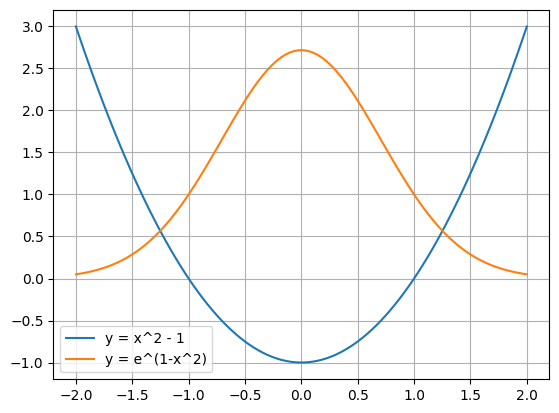
\includegraphics{Deber3_files/figure-pdf/cell-3-output-1.png}

\begin{enumerate}
\def\labelenumi{\arabic{enumi}.}
\setcounter{enumi}{1}
\tightlist
\item
  Use el método de bisección para encontrar una aproximación dentro de
  (10\^{}\{-6\}) para un valor en ({[}-2, 0{]}) con (x - 1 = e\^{}x).
\end{enumerate}

\begin{Shaded}
\begin{Highlighting}[]
\ImportTok{import}\NormalTok{ numpy }\ImportTok{as}\NormalTok{ np}

\KeywordTok{def}\NormalTok{ f(x):}
    \ControlFlowTok{return}\NormalTok{ x}\OperatorTok{**}\DecValTok{2} \OperatorTok{{-}} \DecValTok{1} \OperatorTok{{-}}\NormalTok{ np.exp(}\DecValTok{1}\OperatorTok{{-}}\NormalTok{x}\OperatorTok{**}\DecValTok{2}\NormalTok{)}

\KeywordTok{def}\NormalTok{ biseccion(a, b, tol):}
    \ControlFlowTok{while}\NormalTok{ (b}\OperatorTok{{-}}\NormalTok{a)}\OperatorTok{/}\DecValTok{2} \OperatorTok{\textgreater{}}\NormalTok{ tol:}
\NormalTok{        c }\OperatorTok{=}\NormalTok{ (a}\OperatorTok{+}\NormalTok{b)}\OperatorTok{/}\DecValTok{2}
        \ControlFlowTok{if}\NormalTok{ f(a)}\OperatorTok{*}\NormalTok{f(c) }\OperatorTok{\textless{}} \DecValTok{0}\NormalTok{:}
\NormalTok{            b }\OperatorTok{=}\NormalTok{ c}
        \ControlFlowTok{else}\NormalTok{:}
\NormalTok{            a }\OperatorTok{=}\NormalTok{ c}
    \ControlFlowTok{return}\NormalTok{ (a}\OperatorTok{+}\NormalTok{b)}\OperatorTok{/}\DecValTok{2}

\CommentTok{\# Parámetros iniciales}
\NormalTok{a }\OperatorTok{=} \OperatorTok{{-}}\DecValTok{2}
\NormalTok{b }\OperatorTok{=} \DecValTok{0}
\NormalTok{tol }\OperatorTok{=} \FloatTok{1e{-}3}

\CommentTok{\# Aplicar el método de bisección}
\NormalTok{raiz }\OperatorTok{=}\NormalTok{ biseccion(a, b, tol)}

\BuiltInTok{print}\NormalTok{(}\StringTok{"La raíz aproximada es:"}\NormalTok{, raiz)}
\end{Highlighting}
\end{Shaded}

\begin{verbatim}
La raíz aproximada es: -1.2509765625
\end{verbatim}

\begin{Shaded}
\begin{Highlighting}[]
\ImportTok{import}\NormalTok{ matplotlib.pyplot }\ImportTok{as}\NormalTok{ plt}

\NormalTok{x }\OperatorTok{=}\NormalTok{ np.linspace(}\OperatorTok{{-}}\DecValTok{2}\NormalTok{, }\DecValTok{2}\NormalTok{, }\DecValTok{100}\NormalTok{)}
\NormalTok{y }\OperatorTok{=}\NormalTok{ f(x)}
\NormalTok{plt.plot(x, y)}
\NormalTok{plt.axhline(y}\OperatorTok{=}\DecValTok{0}\NormalTok{, color}\OperatorTok{=}\StringTok{\textquotesingle{}k\textquotesingle{}}\NormalTok{, linestyle}\OperatorTok{=}\StringTok{\textquotesingle{}{-}{-}\textquotesingle{}}\NormalTok{)}
\NormalTok{plt.axvline(x}\OperatorTok{=}\NormalTok{raiz, color}\OperatorTok{=}\StringTok{\textquotesingle{}r\textquotesingle{}}\NormalTok{, linestyle}\OperatorTok{=}\StringTok{\textquotesingle{}{-}{-}\textquotesingle{}}\NormalTok{)}
\NormalTok{plt.show()}
\end{Highlighting}
\end{Shaded}

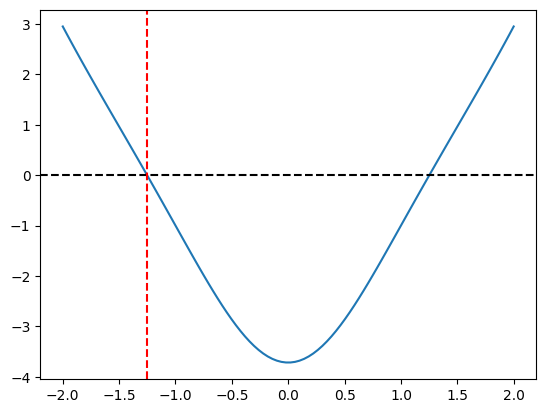
\includegraphics{Deber3_files/figure-pdf/cell-5-output-1.png}

\subsection{Ejercicio 5}\label{ejercicio-5}

Sea \$ f(x) = (x + 3)(x + 1)x(x - 1)(x - 3)\$. ¿En qué cero de (f)
converge el método de bisección cuando se aplica en los siguientes
intervalos?\\
- a. ({[}-1.5, 2.5{]}) - b. {[}−0.5, 2.4{]} - c.~{[}−0.5,3{]} -
d.~{[}−3,−0.5{]}

\begin{Shaded}
\begin{Highlighting}[]
\ImportTok{import}\NormalTok{ numpy }\ImportTok{as}\NormalTok{ np}
\ImportTok{import}\NormalTok{ matplotlib.pyplot }\ImportTok{as}\NormalTok{ plt}

\KeywordTok{def}\NormalTok{ f(x):}
    \ControlFlowTok{return}\NormalTok{ (x}\OperatorTok{+}\DecValTok{3}\NormalTok{)}\OperatorTok{*}\NormalTok{(x}\OperatorTok{+}\DecValTok{1}\NormalTok{)}\OperatorTok{**}\DecValTok{2}\OperatorTok{*}\NormalTok{(x}\OperatorTok{{-}}\DecValTok{1}\NormalTok{)}\OperatorTok{*}\NormalTok{(x}\OperatorTok{{-}}\DecValTok{3}\NormalTok{)}

\KeywordTok{def}\NormalTok{ biseccion(a, b, tol):}
    \ControlFlowTok{while}\NormalTok{ (b}\OperatorTok{{-}}\NormalTok{a)}\OperatorTok{/}\DecValTok{2} \OperatorTok{\textgreater{}}\NormalTok{ tol:}
\NormalTok{        c }\OperatorTok{=}\NormalTok{ (a}\OperatorTok{+}\NormalTok{b)}\OperatorTok{/}\DecValTok{2}
        \ControlFlowTok{if}\NormalTok{ f(a)}\OperatorTok{*}\NormalTok{f(c) }\OperatorTok{\textless{}} \DecValTok{0}\NormalTok{:}
\NormalTok{            b }\OperatorTok{=}\NormalTok{ c}
        \ControlFlowTok{else}\NormalTok{:}
\NormalTok{            a }\OperatorTok{=}\NormalTok{ c}
    \ControlFlowTok{return}\NormalTok{ (a}\OperatorTok{+}\NormalTok{b)}\OperatorTok{/}\DecValTok{2}

\CommentTok{\# Definimos los intervalos}
\NormalTok{intervalos }\OperatorTok{=}\NormalTok{ [[}\OperatorTok{{-}}\FloatTok{1.5}\NormalTok{, }\FloatTok{2.5}\NormalTok{], [}\OperatorTok{{-}}\FloatTok{0.5}\NormalTok{, }\FloatTok{2.4}\NormalTok{], [}\OperatorTok{{-}}\FloatTok{0.5}\NormalTok{, }\DecValTok{3}\NormalTok{], [}\OperatorTok{{-}}\DecValTok{3}\NormalTok{, }\OperatorTok{{-}}\FloatTok{0.5}\NormalTok{]]}

\ControlFlowTok{for}\NormalTok{ intervalo }\KeywordTok{in}\NormalTok{ intervalos:}
\NormalTok{    a, b }\OperatorTok{=}\NormalTok{ intervalo}
    \ControlFlowTok{try}\NormalTok{:}
\NormalTok{        raiz }\OperatorTok{=}\NormalTok{ biseccion(a, b, }\FloatTok{1e{-}6}\NormalTok{)}
        \BuiltInTok{print}\NormalTok{(}\SpecialStringTok{f"Intervalo: }\SpecialCharTok{\{}\NormalTok{intervalo}\SpecialCharTok{\}}\SpecialStringTok{"}\NormalTok{)}
        \BuiltInTok{print}\NormalTok{(}\SpecialStringTok{f"Raíz aproximada: }\SpecialCharTok{\{}\NormalTok{raiz}\SpecialCharTok{\}}\SpecialStringTok{"}\NormalTok{)}
        
        \CommentTok{\# Visualización (opcional)}
\NormalTok{        x }\OperatorTok{=}\NormalTok{ np.linspace(a, b, }\DecValTok{100}\NormalTok{)}
\NormalTok{        y }\OperatorTok{=}\NormalTok{ f(x)}
\NormalTok{        plt.plot(x, y)}
\NormalTok{        plt.axhline(y}\OperatorTok{=}\DecValTok{0}\NormalTok{, color}\OperatorTok{=}\StringTok{\textquotesingle{}k\textquotesingle{}}\NormalTok{, linestyle}\OperatorTok{=}\StringTok{\textquotesingle{}{-}{-}\textquotesingle{}}\NormalTok{)}
\NormalTok{        plt.axvline(x}\OperatorTok{=}\NormalTok{raiz, color}\OperatorTok{=}\StringTok{\textquotesingle{}r\textquotesingle{}}\NormalTok{, linestyle}\OperatorTok{=}\StringTok{\textquotesingle{}{-}{-}\textquotesingle{}}\NormalTok{)}
\NormalTok{        plt.title(}\SpecialStringTok{f"Intervalo: }\SpecialCharTok{\{}\NormalTok{intervalo}\SpecialCharTok{\}}\SpecialStringTok{"}\NormalTok{)}
\NormalTok{        plt.grid(}\VariableTok{True}\NormalTok{)}
\NormalTok{        plt.show()}
    \ControlFlowTok{except}\NormalTok{:}
        \BuiltInTok{print}\NormalTok{(}\SpecialStringTok{f"No se pudo encontrar una raíz en el intervalo }\SpecialCharTok{\{}\NormalTok{intervalo}\SpecialCharTok{\}}\SpecialStringTok{"}\NormalTok{)}
\end{Highlighting}
\end{Shaded}

\begin{verbatim}
Intervalo: [-1.5, 2.5]
Raíz aproximada: 1.4999990463256836
\end{verbatim}

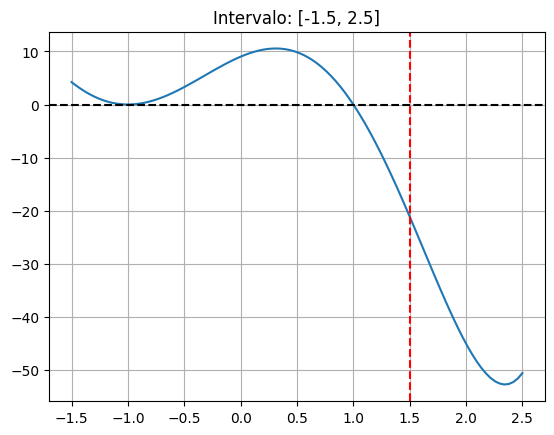
\includegraphics{Deber3_files/figure-pdf/cell-6-output-2.png}

\begin{verbatim}
Intervalo: [-0.5, 2.4]
Raíz aproximada: 0.9999995946884154
\end{verbatim}

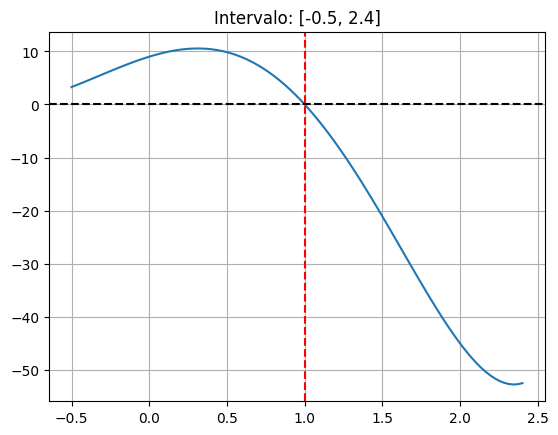
\includegraphics{Deber3_files/figure-pdf/cell-6-output-4.png}

\begin{verbatim}
Intervalo: [-0.5, 3]
Raíz aproximada: 1.0000001192092896
\end{verbatim}

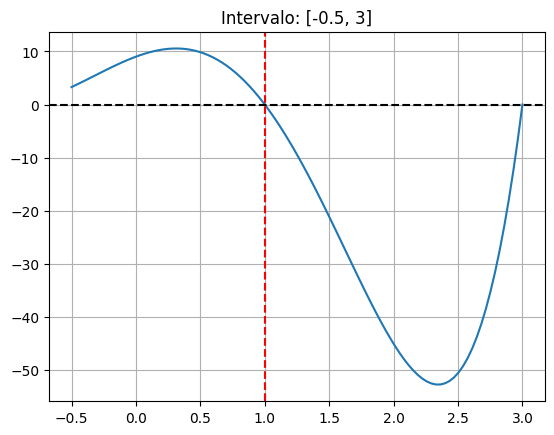
\includegraphics{Deber3_files/figure-pdf/cell-6-output-6.png}

\begin{verbatim}
Intervalo: [-3, -0.5]
Raíz aproximada: -0.5000005960464478
\end{verbatim}

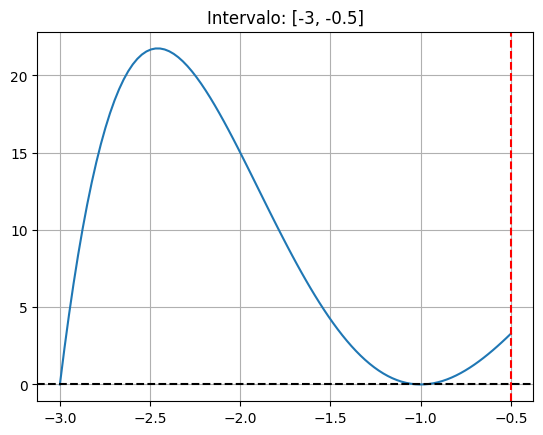
\includegraphics{Deber3_files/figure-pdf/cell-6-output-8.png}

\subsection{Análisis de la Convergencia del Método de
Bisección}\label{anuxe1lisis-de-la-convergencia-del-muxe9todo-de-bisecciuxf3n}

\textbf{Función:} f(x) = (x+3)(x+1)\^{}2(x-1)(x-3)

\subsubsection{Intervalos y Análisis}\label{intervalos-y-anuxe1lisis}

\begin{longtable}[]{@{}llll@{}}
\toprule\noalign{}
Intervalo & f(extremo izquierdo) & f(extremo derecho) & Convergencia \\
\midrule\noalign{}
\endhead
\bottomrule\noalign{}
\endlastfoot
{[}-1.5, 2.5{]} & Positivo & Negativo & Sí \\
{[}-0.5, 2.4{]} & Positivo & Negativo & Sí \\
{[}-0.5, 3{]} & Positivo & 0 & No se puede asegurar \\
{[}-3, -0.5{]} & 0 & Positivo & No se puede asegurar \\
\end{longtable}

\subsubsection{Conclusiones}\label{conclusiones}

\begin{itemize}
\tightlist
\item
  \textbf{Convergencia:} El método de bisección converge en los
  intervalos \textbf{{[}-1.5, 2.5{]}} y \textbf{{[}-0.5, 2.4{]}} ya que
  la función cambia de signo en estos intervalos.
\item
  \textbf{No convergencia:} No se puede asegurar la convergencia en los
  intervalos \textbf{{[}-0.5, 3{]}} y \textbf{{[}-3, -0.5{]}} debido a
  que la función se anula en uno de los extremos.
\end{itemize}

\textbf{Explicación:}

Para que el método de bisección converja, la función debe cambiar de
signo en el intervalo. Esto se debe al teorema del valor intermedio, que
garantiza la existencia de al menos una raíz en el intervalo.

En los casos donde la función se anula en uno de los extremos, no
podemos asegurar la convergencia ya que el método de bisección asume que
la función cambia de signo en todo el intervalo.

\section{Ejercicios Aplicados}\label{ejercicios-aplicados}

\subsection{Ejercicio 1}\label{ejercicio-1-1}

Un abrevadero de longitud (L) tiene una sección transversal en forma de
semicírculo con radio (r). (Consulte la figura adjunta.) Cuando se llena
con agua hasta una distancia (h) a partir de la parte superior, el
volumen (V) de agua es:\\
\[
V = L \left[ 0.5 \pi r^2 - r^2 \arcsin\left(\frac{h}{r}\right) - h \sqrt{r^2 - h^2} \right]
\]

Suponga que L = 10 cm, r = 1 cm y V = 12.4 cm\^{}3. Encuentre la
profundidad del agua en el abrevadero dentro de 0.01 cm.

\subsection{Resolución del Problema}\label{resoluciuxf3n-del-problema}

\subsubsection{Paso 1: Planteamiento del
problema}\label{paso-1-planteamiento-del-problema}

Dado: - ( L = 10 , \text{cm} ) - ( r = 1 , \text{cm} ) - ( V = 12.4 ,
\text{cm}\^{}3 )

Queremos encontrar ( h ) tal que: {[} V = L
\left[ 0.5 \pi r^2 - r^2 \arcsin\left(\frac{h}{r}\right) - h \left( r^2 - h^2 \right)^{1/2} \right]{]}

\subsubsection{Paso 2: Definir la función a
resolver}\label{paso-2-definir-la-funciuxf3n-a-resolver}

Restamos el volumen dado a la ecuación y definimos una nueva función (
f(h) ) como:

{[} f(h) = L
\left[ 0.5 \pi r^2 - r^2 \arcsin\left(\frac{h}{r}\right) - h \left( r^2 - h^2 \right)^{1/2} \right] -
V {]}

La solución se encuentra cuando ( f(h) = 0 ).

\subsubsection{Paso 3: Elegir un intervalo inicial para ( h
)}\label{paso-3-elegir-un-intervalo-inicial-para-h}

Sabemos que ( h ) debe estar entre 0 y ( r ), porque la profundidad no
puede ser mayor que el radio del semicírculo. Por lo tanto, nuestro
intervalo inicial podría ser algo como ( {[}0, 1{]} ).

\subsubsection{Paso 4: Implementar el método de
bisección}\label{paso-4-implementar-el-muxe9todo-de-bisecciuxf3n}

El método de bisección encuentra una raíz de la función dentro de un
intervalo ( {[}a, b{]} ). Se calcula el punto medio ( c ) del intervalo
y se verifica el signo de ( f(c) ):

\begin{itemize}
\tightlist
\item
  Si ( f(a) ) y ( f(c) ) tienen signos diferentes, la raíz se encuentra
  en ( {[}a, c{]} ).
\item
  Si ( f(c) ) y ( f(b) ) tienen signos diferentes, la raíz se encuentra
  en ( {[}c, b{]} ).
\end{itemize}

Este proceso se repite hasta que la diferencia entre los extremos ( a )
y ( b ) sea menor que la tolerancia requerida, en este caso, ( 0.01 ,
\text{cm} ).

\begin{Shaded}
\begin{Highlighting}[]
\ImportTok{import}\NormalTok{ math}

\KeywordTok{def}\NormalTok{ volumen(h, L, r):}
    \ControlFlowTok{return}\NormalTok{ L }\OperatorTok{*}\NormalTok{ (}\FloatTok{0.5} \OperatorTok{*}\NormalTok{ math.pi }\OperatorTok{*}\NormalTok{ r}\OperatorTok{**}\DecValTok{2} \OperatorTok{{-}}\NormalTok{ r}\OperatorTok{**}\DecValTok{2} \OperatorTok{*}\NormalTok{ math.asin(h }\OperatorTok{/}\NormalTok{ r) }\OperatorTok{{-}}\NormalTok{ h }\OperatorTok{*}\NormalTok{ math.sqrt(r}\OperatorTok{**}\DecValTok{2} \OperatorTok{{-}}\NormalTok{ h}\OperatorTok{**}\DecValTok{2}\NormalTok{))}

\KeywordTok{def}\NormalTok{ biseccion(L, r, V, tol}\OperatorTok{=}\FloatTok{0.01}\NormalTok{):}
\NormalTok{    a }\OperatorTok{=} \DecValTok{0}
\NormalTok{    b }\OperatorTok{=}\NormalTok{ r}
    \ControlFlowTok{while}\NormalTok{ (b }\OperatorTok{{-}}\NormalTok{ a) }\OperatorTok{/} \FloatTok{2.0} \OperatorTok{\textgreater{}}\NormalTok{ tol:}
\NormalTok{        c }\OperatorTok{=}\NormalTok{ (a }\OperatorTok{+}\NormalTok{ b) }\OperatorTok{/} \FloatTok{2.0}
        \ControlFlowTok{if}\NormalTok{ (volumen(c, L, r) }\OperatorTok{{-}}\NormalTok{ V) }\OperatorTok{==} \DecValTok{0}\NormalTok{:}
            \ControlFlowTok{return}\NormalTok{ c}
        \ControlFlowTok{elif}\NormalTok{ (volumen(a, L, r) }\OperatorTok{{-}}\NormalTok{ V) }\OperatorTok{*}\NormalTok{ (volumen(c, L, r) }\OperatorTok{{-}}\NormalTok{ V) }\OperatorTok{\textless{}} \DecValTok{0}\NormalTok{:}
\NormalTok{            b }\OperatorTok{=}\NormalTok{ c}
        \ControlFlowTok{else}\NormalTok{:}
\NormalTok{            a }\OperatorTok{=}\NormalTok{ c}
    \ControlFlowTok{return}\NormalTok{ (a }\OperatorTok{+}\NormalTok{ b) }\OperatorTok{/} \FloatTok{2.0}

\CommentTok{\# Parámetros dados}
\NormalTok{L }\OperatorTok{=} \DecValTok{10}  \CommentTok{\# longitud en cm}
\NormalTok{r }\OperatorTok{=} \DecValTok{1}   \CommentTok{\# radio en cm}
\NormalTok{V }\OperatorTok{=} \FloatTok{12.4}  \CommentTok{\# volumen en cm\^{}3}

\CommentTok{\# Llamar a la función de bisección para encontrar h}
\NormalTok{profundidad }\OperatorTok{=}\NormalTok{ biseccion(L, r, V)}
\BuiltInTok{print}\NormalTok{(}\SpecialStringTok{f"La profundidad h es aproximadamente: }\SpecialCharTok{\{}\NormalTok{profundidad}\SpecialCharTok{:.2f\}}\SpecialStringTok{ cm"}\NormalTok{)}
\end{Highlighting}
\end{Shaded}

\begin{verbatim}
La profundidad h es aproximadamente: 0.16 cm
\end{verbatim}

\subsection{Ejercicio 2}\label{ejercicio-2}

Un objeto que cae verticalmente a través del aire está sujeto a una
resistencia viscosa, así como a la fuerza de gravedad. Suponga que un
objeto con masa (m) cae desde una altura (s) y que la altura del objeto
después de (t) segundos es:\\
\[
s(t) = s_0 - \frac{mg}{k} + \frac{m^2g}{k^2}\left( 1 - e^{-kt} \right)
\]

donde 𝑔 = 9.81 𝑚/𝑠 y 𝑘 representa el coeficiente de la resistencia del
aire en 𝑁𝑠 /𝑚. Suponga 𝑠 = 300 𝑚,\\
m=0.25 𝑘𝑔 y 𝑘 = 0.1𝑁𝑠 𝑚. Encuentre, dentro de 0.01 𝑠𝑒𝑔𝑢𝑛𝑑𝑜𝑠, el tiempo
que tarda un cuarto de kg en golpear el piso.

\begin{Shaded}
\begin{Highlighting}[]
\ImportTok{import}\NormalTok{ numpy }\ImportTok{as}\NormalTok{ np}
\ImportTok{from}\NormalTok{ scipy.optimize }\ImportTok{import}\NormalTok{ fsolve}

\KeywordTok{def}\NormalTok{ equation(t):}
\NormalTok{  s0 }\OperatorTok{=} \DecValTok{300}
\NormalTok{  m }\OperatorTok{=} \FloatTok{0.25}
\NormalTok{  g }\OperatorTok{=} \FloatTok{9.81}
\NormalTok{  k }\OperatorTok{=} \FloatTok{0.1}
  \ControlFlowTok{return}\NormalTok{ s0 }\OperatorTok{{-}}\NormalTok{ (m}\OperatorTok{*}\NormalTok{g}\OperatorTok{/}\NormalTok{k)}\OperatorTok{*}\NormalTok{t }\OperatorTok{+}\NormalTok{ (m}\OperatorTok{**}\DecValTok{2}\OperatorTok{*}\NormalTok{g}\OperatorTok{/}\NormalTok{k}\OperatorTok{**}\DecValTok{2}\NormalTok{)}\OperatorTok{*}\NormalTok{(}\DecValTok{1} \OperatorTok{{-}}\NormalTok{ np.exp(}\OperatorTok{{-}}\NormalTok{k}\OperatorTok{*}\NormalTok{t}\OperatorTok{/}\NormalTok{m))}

\CommentTok{\# Improved initial guess based on the physics of the problem (assuming object starts from rest)}
\NormalTok{initial\_guess }\OperatorTok{=} \DecValTok{10}  \CommentTok{\# Adjust as needed}

\CommentTok{\# Try with adjusted tolerance for xtol}
\NormalTok{root }\OperatorTok{=}\NormalTok{ fsolve(equation, initial\_guess, xtol}\OperatorTok{=}\FloatTok{1e{-}6}\NormalTok{)}
\BuiltInTok{print}\NormalTok{(}\StringTok{"El tiempo que tarda en golpear el suelo es:"}\NormalTok{, root[}\DecValTok{0}\NormalTok{], }\StringTok{"segundos"}\NormalTok{)}
\end{Highlighting}
\end{Shaded}

\begin{verbatim}
El tiempo que tarda en golpear el suelo es: 14.725499843314939 segundos
\end{verbatim}

\section{Ejercicios Teóricos}\label{ejercicios-teuxf3ricos}

\subsection{Ejercicio 1}\label{ejercicio-1-2}

Use el teorema 2.1 para encontrar una cota para el número de iteraciones
necesarias para lograr una aproximación con precisión de (10\^{}\{-6\})
para la solución de (x\^{}2 - x - 1 = 0) que se encuentra dentro del
intervalo ({[}1, 2{]}). Encuentre una aproximación para la raíz con este
grado de precisión.

\begin{Shaded}
\begin{Highlighting}[]
\KeywordTok{def}\NormalTok{ f(x):}
  \CommentTok{"""Función a evaluar"""}
  \ControlFlowTok{return}\NormalTok{ x}\OperatorTok{**}\DecValTok{2} \OperatorTok{{-}}\NormalTok{ x }\OperatorTok{{-}} \DecValTok{1}

\KeywordTok{def}\NormalTok{ biseccion(a, b, tol):}
  \CommentTok{"""Método de bisección para encontrar una raíz"""}
\NormalTok{  n }\OperatorTok{=} \DecValTok{0}
  \ControlFlowTok{while}\NormalTok{ (b}\OperatorTok{{-}}\NormalTok{a)}\OperatorTok{/}\DecValTok{2} \OperatorTok{\textgreater{}}\NormalTok{ tol:}
\NormalTok{    p }\OperatorTok{=}\NormalTok{ (a}\OperatorTok{+}\NormalTok{b)}\OperatorTok{/}\DecValTok{2}
    \ControlFlowTok{if}\NormalTok{ f(p) }\OperatorTok{==} \DecValTok{0}\NormalTok{:}
      \ControlFlowTok{break}
    \ControlFlowTok{elif}\NormalTok{ f(a)}\OperatorTok{*}\NormalTok{f(p) }\OperatorTok{\textless{}} \DecValTok{0}\NormalTok{:}
\NormalTok{      b }\OperatorTok{=}\NormalTok{ p}
    \ControlFlowTok{else}\NormalTok{:}
\NormalTok{      a }\OperatorTok{=}\NormalTok{ p}
\NormalTok{    n }\OperatorTok{+=} \DecValTok{1}
  \ControlFlowTok{return}\NormalTok{ p, n}

\CommentTok{\# Parámetros iniciales}
\NormalTok{a }\OperatorTok{=} \DecValTok{1}
\NormalTok{b }\OperatorTok{=} \DecValTok{2}
\NormalTok{tol }\OperatorTok{=} \FloatTok{1e{-}5}

\CommentTok{\# Aplicar el método de bisección}
\NormalTok{raiz, iteraciones }\OperatorTok{=}\NormalTok{ biseccion(a, b, tol)}

\CommentTok{\# Imprimir resultados}
\BuiltInTok{print}\NormalTok{(}\StringTok{"La aproximación de la raíz es:"}\NormalTok{, raiz)}
\BuiltInTok{print}\NormalTok{(}\StringTok{"Número de iteraciones:"}\NormalTok{, iteraciones)}
\end{Highlighting}
\end{Shaded}

\begin{verbatim}
La aproximación de la raíz es: 1.6180267333984375
Número de iteraciones: 16
\end{verbatim}




\end{document}
